\documentclass{article}
\usepackage[table]{xcolor}
\usepackage[paper=letterpaper,left=1.2cm,right=1.2cm,top=2cm,bottom=1cm,includefoot]{geometry}
\usepackage{tabularx}
\usepackage{multirow}
\usepackage{hyperref}
\usepackage{hhline}
\usepackage{amsmath}
\usepackage{enumitem}
\usepackage{pgfgantt}
\usepackage{graphicx}   \graphicspath{{img/}}
\usepackage{float}
\usepackage{fancyhdr}
% \usepackage{subfigure} 

\usepackage{caption}
\usepackage{subcaption, booktabs}
\usepackage[spanish]{babel}
\usepackage[utf8]{inputenc}


%%% Comente/Descomente las siguientes lineas para cambiar la fuente del texto
%\usepackage{DejaVuSans}
%\renewcommand*\familydefault{\sfdefault}
\usepackage{sansmath}
\sansmath

\usepackage{xcolor}
\definecolor{LightGray}{gray}{0.92}
% \usepackage{minted}
% \newminted{python}{ linenos,breaklines,mathescape,texcomments,xleftmargin=\parindent, numbersep=8pt,  bgcolor=LightGray}
% pdflatex -shell-escape propuesta.tex  comando para usar minted.     
% \renewcommand\listingscaption{C\'odigo}




\pagestyle{empty}

\definecolor{tcc}{RGB}{217,217,217} % Table cell color

\renewcommand\tabularxcolumn[1]{m{#1}}
\setlength{\arrayrulewidth}{0.5pt}
\renewcommand{\arraystretch}{2}

\renewcommand{\thesection}{\alph{section})}
\renewcommand{\thesubsection}{\alph{section}.\arabic{subsection}}

\renewcommand{\refname}{\vspace{-2ex}}




\lhead{\begin{picture}(0,0)\put(0,0){
\includegraphics[width=10mm]{LogoU.jpeg}} \end{picture}}
\chead{Facultad de Ciencias Físicas y Matemáticas\\ Departamento de Física}
\rhead{Proyecto: "Fight Club"}
\renewcommand{\headrulewidth}{0.5pt}

\pagestyle{fancy}





\begin{document}

\begin{center}
\begin{huge}
\textbf{Estudio sobre particulas atrapadas}
\end{huge}
\vspace*{0.01cm}
\end{center}





\textbf{Integrantes:} Eduardo Escudero
\textbf{Fecha:} \today


\hspace{4cm}


\begin{center}
\rule{12cm}{0.1mm}
\end{center}














%%%%%%%%%%%%%%%%%%%%%%%%%%%%%%----Abstract o propuesta de proyecto-----%%%%%%%%%%%%%%%%%%%%%%%%%%%%%%%%%%%%%%%%%%%%%%%%%%

\begin{abstract}

En el presente proyecto se buscará crear un repositorio de informacion sobre particulas atrapadas, partiendo por el estudio teorico
para darle un enfoque experimental, generando un camino y una via de fácil estudio. Para estos tópicos de la Física contemporanea.

\end{abstract}

%%%%%%%%%%%%%%%%%%%%------Objetivos de proyecto----%%%%%%%%%%%%%%%%%%%%%%%%%%%%%%%%%%%%%%%%%%%%%%%%%%%%%%%%%%%%



\section*{Objetivos de trabajo}


\subsection*{Objetivo general}

El objetivo de este repositorio/bitácora es generar el conocimiento necesario para poder empezar o ser de utilidad dentro de un laboratorio de 
fisica experimental, principalmente los topicos van a ser centrados en fisica de particulas atrapadas. Dado mi propio interes como editor, pero con 
vistas a un publico general de física experimental.

\section*{Proyectos y explicaciones}
Lo que buscaria es poder tener diferentes proyectos y poder ir agregandolos poco a poco aqui de manera sirvan como guia de estudio para la gente que
este interesada en seguir este campo de estudio.
\subsection*{"Trampa Paul" o "Paul Trap"}
En este primer proyecto vamos a estudiar la trampa de Paul, la cual consiste basicamente en la manera más común de atrapar atomos o más específicamente íones
el principio es bastante básico, dado la existencia de las cargas en un íon este puede ser encapsulado por gradientes electricos al generar un punto de menor 
energia, esto va a permitir que 
\begin{enumerate}
\item Estudiar principios físicos de la trampa de Paul

\item Estudiar modelos actuales de la trampa de Paul

\item Crear una simulación de una trampa de Paul funcional

\end{enumerate}


%%%%%%%%%%%%%%%%%%%%%---Metodologia o procedimiento--%%%%%%%%%%%%%%%%%%%%%%%%%%%%%%%%%%%%%%%%%%%%%%%%%%%%%%%%%%%

\subsubsection*{Metodología}

Para demostrar como cumplidos estos objetivos lo que vamos a buscar demostrar es poder encontrar los modos normales
y las situaciones de equilibrio para 1, 2 y 3 iones atrapados. Los primero de manera
analítica y la última de manera numérica. Finalmente compararemos estos dos resultados para 
poder calcular el margen de nuestra simulación y de nuestros cálculos.

El método de para poder hacer el cálculo numérico que se hará será Rhunge Kutta, el cuál es un
método destinado a poder cálcular sistemas de ecuaciones diferenciales lo cual es especialmente
útil en la resolución de problemas matemáticos \cite{Rhunge-Kutta}, es conocido 
por ser un método lineal de un paso, lo que significa que solo necesita un punto para 
empezar a crear una estimación.

Lo que se espera ver durante nuesto estudio es que existan modos normales, equivalentes
a sistemas acoplados por lo que finalmente en el modelo de 2 iones encontraremos 2 modos normales
por cada orden de libertad, para el modelo de 3 iones encontraremos 3 modos por cada orden. Asi como section
se puede apreciar en la figuara \ref{fig:sistemasacoplados} donde podemos ver los modos que
deberiamos encontrar en los tres objetivos impuestos y buscaremos cuales son las condiciones
necesarias para que esto se cumpla.

%---------------------------------------------------------------%
\begin{figure}
    \centering
    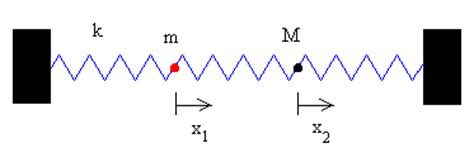
\includegraphics[width=0.5\textwidth]{sis_aco1.jpeg}
    \caption{Sistema de resortes acoplados, sus modos normales y sus puntos de equilibrio como hipotesis a encontrar en el comportamiento de "Paul Trap" ó "Trampa de Paul"}
    \label{fig:sistemasacoplados}
\end{figure}
% \begin{figure}
%     \centering
%     \includegraphics[width=0.5\textwidth]{a2.jpeg}
%     % \caption{Sistema de resortes acoplados, sus modos normales y sus puntos de equilibrio como hipotesis a encontrar en el comportamiento de "Paul Trap" ó "Trampa de Paul"}
% \end{figure}
%------------------------Idea 1---------------------------------------%
\subsubsection*{Principios de la "Trampa de Paul" ó "Paul Trap"}

Primero que nada Wolfgang Paul es  uno de los investigadores principales de el descubrimiento de la trampa
de Paul, es por ello que esta lleva su nombre. La cuál consiste en una trampa cuadripolar
la cuál fue acreedora del premio nobel de física en 1989.\cite{hist_paul}

Para poder entender como funciona la trampa de Paul debemos edntender como es la física
entre átomos atrapados, lo que se sabe es que independientemente de que los átomos 
no presenten alguna carga predominante o iones estos presentan interecaciones más 
débiles por lo que se puede decir que en partículas atrapadas va a existir una fuerza
vinculante ($F_{vin}$) que va a mantener "unidos" hasta cierto punto a los átomos la cuál
crece con la distancia.$F_{vin}=-cr$
%------------------------Fig---------------------------------------%

\begin{figure}\label{fuerza_vinculante}
    \centering
    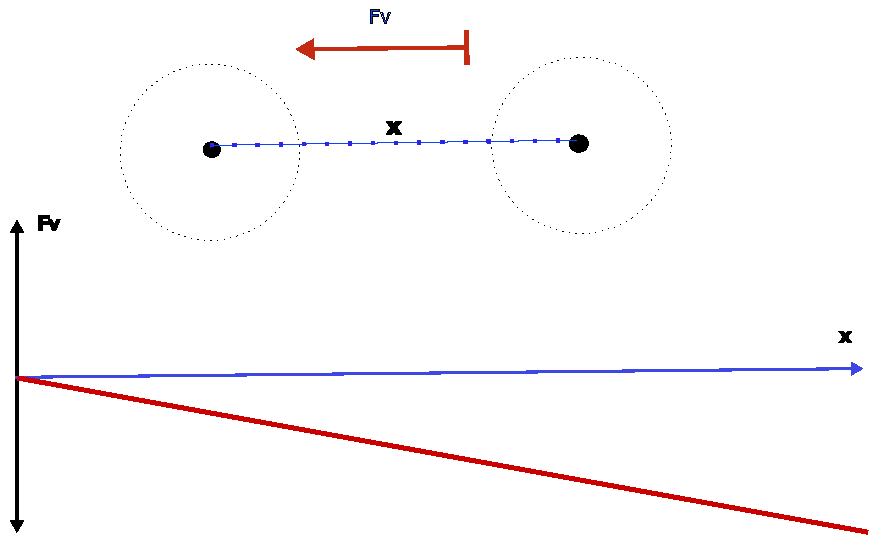
\includegraphics[width=0.4\textwidth]{atomos.pdf}
    \caption{el gráfico indica que a medida que los átomos se alejen la fuerza vinculante va a tender al crecimiento, con ciertos limites debido a la propia repulsión de los mismos. }
\end{figure}

%-------------------------------------------------------------------%

Dado este comportamiento lineal de la fuerza vinculante podemos gracias a la relación de campos
conservativos con los potenciales y la fuerza\eqref{Campo_conservativo} que el potencial($\Phi$) de esta 
fuerza vinculante va a adoptar una forma aproximativa\eqref{forma_potencial} a una parabola cuadratica La
cual trabajando con las simetrias podemos adopatar la expresion\eqref{potencia_rm} donde $m$ es el número de plos o órdenes de
simetriaa de el potencial dado


\begin{equation}\label{Campo_conservativo}
    F(x)=-\frac{dU(x)}{dx}=\frac{d\Phi}{dx}
\end{equation}

\begin{align}
    \Phi    &\approx \alpha x^2+\beta y^2+\gamma z^2\label{forma_potencial} \\
    \Phi    &= r^{m/2}\cos{m/2\phi} \label{potencia_rm}\\
\end{align}

%--------------------------Idea 2-------------------------------------%
\subsubsection*{Atrapando partículas cargadas en 2 y 3 dimensiones}

Teniendo ya un idea de como nuestros átomos van a actuar podemos pasar a 
entender de mejor manera como funciona la trampa de átomos planteada por Paul
la cuál esta pensada principalmente en el uso de iones.

Entonces ahora lo que queremos construir son barreras de potenciales las 
cuales nos van a servir como las paredes de un vaso para mantener al interior
al átomo y es aqui donde entra estos campos cuadripolares, el cuál para nuestra
geometría va a estar representado con la ecuación \eqref{form_cuadripole} la cuál
va estar generada por un potencial inicial($\Phi$), generado por una f.e.m (fuente electro motriz)
y va variar dependiendo de la cercanía de los electrodos ($r_0$).

\begin{equation}
    \Phi=\frac{\Phi_0}{r_0^2}(\alpha x^2+\beta y^2+\gamma z^2)
\end{equation}

Ahora este es el comportamiento que queremos que cumple pero cuáles son las condiciones para 
que esto se cumpla?, para debemos recurrir a tecnicas matemáticas en este caso, al tender a una
forma circular dado \eqref{potencia_rm} optamos por usar la ecuación de Laplace $\Delta \Phi = 0$
la cuál va a imponer que $\alpha + \beta + \gamma=0$ la cuál tiene dos soluciones simples que nos interesan
\begin{itemize}
    \item $\alpha=1=-\gamma, \beta=0$ lo que significa que seria un campo bidimensional ya que una de las componentes es $0$ \eqref{Potencial_2D}
    \item $\alpha=\beta, \gamma=-2$ generando una configuración tridimensional, que puede ser reescrita en coordenadas cílindricas con la condición de $2z_0^0=r_0$ \eqref{Potencial_3D}
\end{itemize}

\begin{align}
    \Phi = \frac{\Phi^0(r^2-2z^2)}{r_0^2+2z_0^2} \hspace{1.5cm} 2z_o^2=r_0^2 \label{Potencial_3D}\\
    \Phi = \frac{\Phi_0}{2r_0^2}(x^2-z^2) \label{Potencial_2D}
\end{align}

%---------------------------------------------------------------%

%---------------------------------------------------------------%
\begin{thebibliography}{5}
    \bibitem{Rhunge-Kutta}\url{https://www.mathstools.com/section/main/Metodos_de_Runge_Kutta?lang=es}
    \bibitem{Paul_nobel}Prof. Dr. Wolfgang Paul (1990). Electromagnetic Traps for Charged and Neutral Particles (Nobel Lecture). , 29(7), 739–748. doi:10.1002/anie.199007391 
    \bibitem{hist_paul}\url{https://pubs.aip.org/physicstoday/Online/5813/Wolfgang-Paul}
\end{thebibliography}

\end{document}